\section{Энгийн өрөөний байршуулалт}
Олон өрөө тасалгаатай орчныг тоглоомд үүсгэдэг энгийн арга. Процедурт аргаар тоглоомын орчныг үүсгэж сурах гэж байгаа бол энэ аргаас эхэлбэл тохиромжтой.

\subsection{Энгийн өрөө байршуулалтын хэрэгжүүлэлт \cite{PMGT}}
\begin{enumerate}
	\item Орчныг ханаар дүүргэнэ
	\item Санамсаргүйгээр өрөөний байршлыг сонгоно.
	      \begin{enumerate}\item
		            Хэрвээ энд аль хэдийн өрөө байхгүй бол өрөөг нэмнэ.
	      \end{enumerate}
	\item Шаардлагад хүрэх хүртэл алхам 2-г давтана.
	\item Нэмсэн өрөөнүүдээ коридороор  холбоно.
\end{enumerate}

\section{BSP}
Энгийн өрөөний байршуулалттай төстэй ба бүтэн нэр нь Binary Space Partitioning. Энэ аргад орон зайг partitioning хийх буюу орон зайны хуваалт хийдэг.  Орон зайг хуваах алгоритмууд ихэвчлэн шаталсан байдлаар ажилладаг. Орон зайн хуваалт нь нүд бүрийг ижил алгоритмаар рекурсив байдлаар хуваах ба энэ нь өгөгдлийг орон зайг space-partitioning tree буюу орон зайн хуваалтын мод бүтцэд зохион байгуулах боломжийг олгоно.

\subsection*{Space-Partitioning Tree}
Уг бүтцээр орон зайн доторх аль ч цэгийн геометр хайлтыг хурдан хийдэг. Энэ нь компьютер графикт Space-Partitioning Tree бүтцийг  онцгой ач холбогдолтой болгох ба raycasting, frustum culling мөн collision detection-г үр ашигтай хийх боломжийг олгоно.

Хамгийн түгээмэл орон зайн хуваалтын арга нь Binary Space Tree. Уг аргад орон зайн нүдийг рекурсив байдлаар хоёр хуваадаг. Ингэснээр орон зай нь Binary Tree буюу хоёртын модон хэлбэрээр төлөөлөгдөх боломжийг олгодог. Хоёртын мод нь цаашлаад үр ашигтай өгөгдлийн хайлт, хадгалалт зэргийг хийх боломжийг олгоно. Space-Partitioning-д хоёртын модноос гадна дөрөвтийн мод эсвэл наймтын мод зэрэг өөр хэлбэрээр хэрэгжүүлж болдог.

Space-Partitioning-г зургийн pixel-н мэдээллийг үр ашигтай хадгалахад ашиглаж болно Зураг \ref{fig:PixelPartition}.
\begin{figure}[t]
	\centering
	\caption{Pixel хуваалт}
	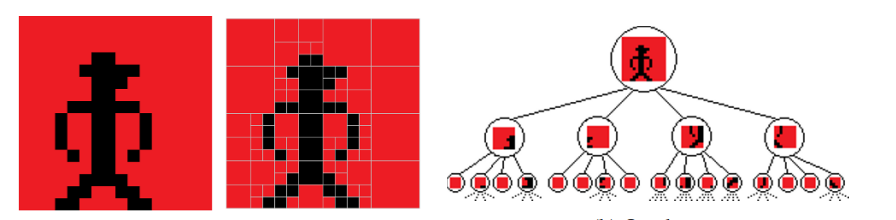
\includegraphics[width=\textwidth]{./images/pixel_partition.png}
	\label{fig:PixelPartition}
\end{figure}

Зураг \ref{fig:PixelPartition}-д: хоёртын зургийг орон зайн дөрөвтийн хуваалт хийсэн. Нэг өнгийн томоохон хэсгүүд болох баруун талын хэсэг нь цаашид хуваалт хийгдээгүй байна. Зураг нь 16x16 харьцаатай ба дөрөвтийн модны гүн нь дөрөв(дөрөвтийн мод \(2^n\) хэмжээтэй мэдээллийг илтгэж чадна. Энд n-н нь модны гүн)
Space-Partitioning аргын давхардсан орон зайн хэсэг үүсгэдэггүй, орон зайг салгадаг зарчим нь олон өрөө тасалгааны бүтцийг гаргахад үр дүнтэй арга \cite{PCGinGames2016}.

Уг арга нь тоглоомын орчныг үүсгэх макро арга ба дээрээс доошоо ажиллах зарчимтай. Өөрөөр хэлбэл уг шийдэл нь орчны хэмжээ хязгаарын мэдээлэл дээр тулгуурлаж хуваалтаа хийдэг.
\subsection{Өрөө тасалгааг BSP-р үүсгэх үйл явц}
\begin{figure}[H]
	\centering
	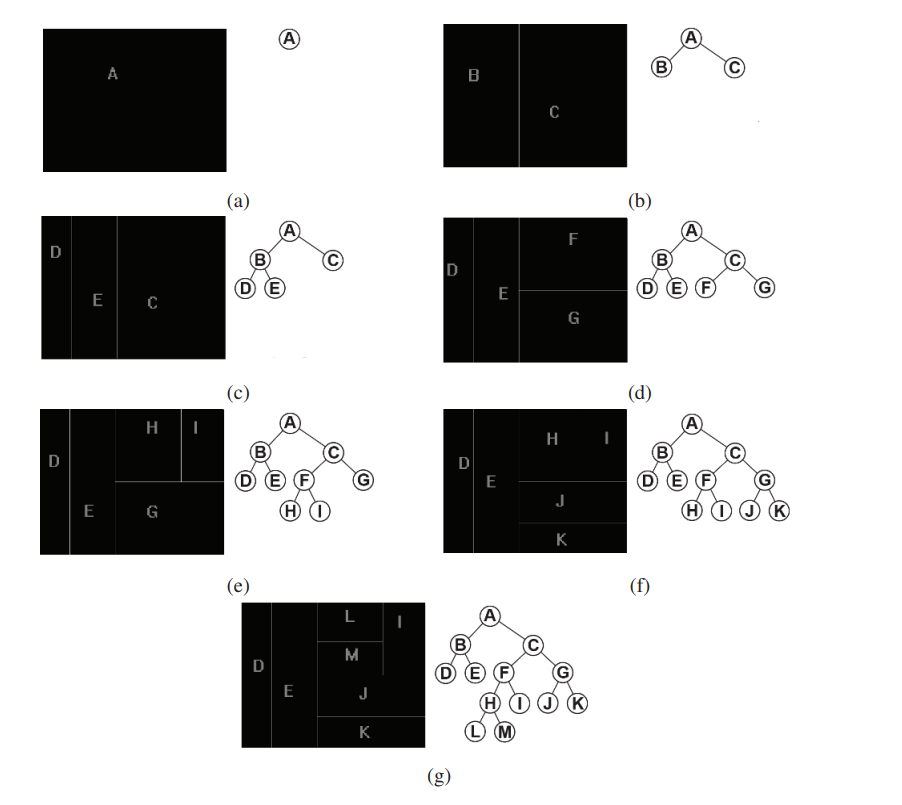
\includegraphics[width=\textwidth]{./images/BSP.png}
	\caption{Өрөө тасалгааны бүтцийг BSP-г үүсгэх үйл явц}
	\label{fig:BSP}
\end{figure}

\begin{enumerate}
	\item Орчны орон зайг бүхлээр нь авна - BSP-н үндэс хэсэг.
	\item Орон зайг босоо эсвэл хэвтээгээр хуваана.
	\item Хуваагдсан хэсгүүдийн нэгийг нь сонгоно
	\item Хэрвээ уг хэсэг нь хамгийн жижиг хэмжээнээс их бол
	\item \quad уг хэсгээр 2 дахь алхам руу явна.
	\item Нөгөө хэсгийг сонгоод 4 дэх алхам руу явна.
	\item Бүх хуваалтын хэсэг болгонд:
	\item \quad Хэсгийн хил дотор санамсаргүйгээр өрөө үүсгэнэ.
	\item Хамгийн доод талын давхаргаас эхлээд адилхан эцэгтэй хэсгүүдийг хооронд нь коридороор  холбоно.
	\item Бүх хэсэг холбогдох хүртэл алхам 9-г давтана.
\end{enumerate}

\begin{figure}[H]
	\centering
	\caption{BSP-н өгөгдлийн бүтцийг ашиглан өрөөнүүдийг коридороор  холбох.}
	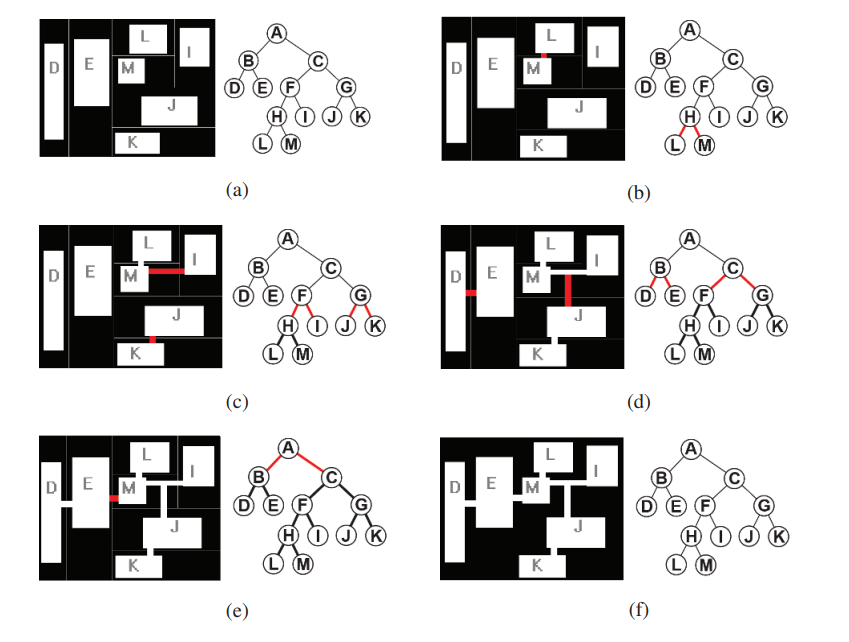
\includegraphics[width=\textwidth]{./images/BSP_connecting.png}
	\label{fig:BSP_connecting}
\end{figure}
Зураг \ref{fig:BSP_connecting}-н зарчмаар өрөөнүүдийг холбосноор хаалганы оноолт нь зөв, аль ч өрөөнөөс өөр аль ч өрөө рүү явах боломжийг олгоно\cite{PCGinGames2016}.

\section{Cellular automata}
\begin{figure}[H]
	\centering
	\caption{2 хэмжээст cellular automata-н хэрэгжүүлэлтийн загвар}
	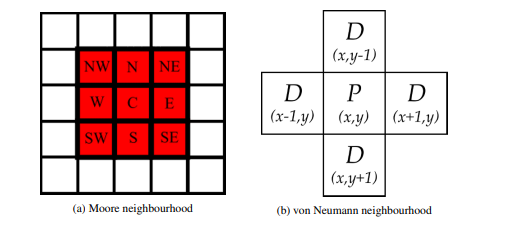
\includegraphics[width=\textwidth]{./images/cellular_automata.png}
	\label{fig:CellularAutomata}
\end{figure}

Cellular Automata-н салангид тооцооллын загвар ба компьютерын ухаан, биологи, физик олон шинжлэх ухааны салбарт өргөн хэлбэрээр судалсан байдаг. Гол ухагдахуун болон алгоритм нь цөөхөн алхамтай.

Жишээ нь:
Cell буюу нэгж нь хоёр төлөвтэй ба үүнд хана эсвэл хоосон зай байна гэж үзье.
\(n\) алхмын турш аливаа нэгж нь хөрш нэгжээсээ шалтгаалж өөрийнхөө төлөвийг өөрчилнө. Түгээмэл хоёр хэмжээст cell automata-н хэрэгжүүлэлтийн загварыг Зураг \ref{fig:CellularAutomata}-г үзүүлэв. Зураг \ref{fig:CellularAutomata}b-д\cite{PCGinGames2016} P-нь одоогийн нэгж ба D нь хөрш нэгж, нэгжийн төлөвийг тодорхойлохдоо хана үүсэх нөхцөлийг 5-с(\(T=5\)) доошгүй хөрш нэгж нь хана байвал P нэгж өөрөө хана болно гэж тодорхойлж болно. Гэхдээ уг давталтыг хийхийн өмнө орчны нэгжүүдэд санамсаргүй байдлаар хана эсвэл хоосон зайн төлөвийг оноож өгөх хэрэгтэй ба үүнд аливаа нэгж нь хана болох боломж \(r=0.5\) гэж үзэж болно.

Johnson et al. \cite{CellularAutomata} дээр \(n=4, T=5, r=0.5, M=1\)(Улаан ханы зузаан) хувьсагчуудаар Cellular Automata ашиглан тоглоомыг орчныг үүсгэсэн Зураг \ref{fig:CellularAutomataImplementation}. Зураг \ref{fig:CellularAutomataImplementation}a дээр нэгжүүдэд анхны санамсаргүй байдлаар төлвүүдийг оноож өгсөн, Зураг \ref{fig:CellularAutomataImplementation}b дээр Cellular Automata-н үйл явцыг \(n=4\) удаа давтсаны дараах үр дүн.
\begin{figure}[H]
	\centering
	\caption{Тоглоомын орчин, Cellular automata-н хэрэгжүүлэлт}
	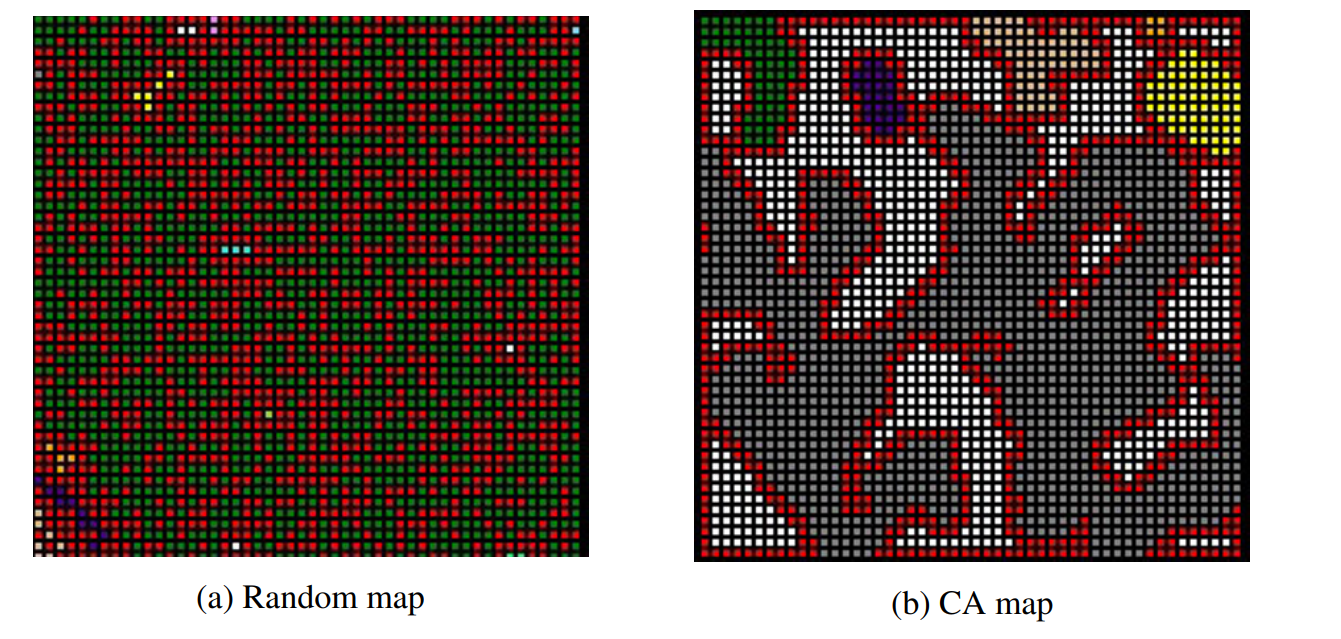
\includegraphics[width=\textwidth]{./images/cellular_automata_implementation.png}
	\label{fig:CellularAutomataImplementation}
\end{figure}

Уг аргаар органик мэт газар доорх тоглоомын орчныг үүсгэх боломжтой. Гэхдээ энэ аргын нэг дутагталтай тал нь хувьсагчуудын утгыг өөрчлөхөд үр дүнг урьчилан мэдэхэд хэцүү.


